

% Gradient Info
  
\tikzset {_jfsff6evj/.code = {\pgfsetadditionalshadetransform{ \pgftransformshift{\pgfpoint{0 bp } { 0 bp }  }  \pgftransformscale{1 }  }}}
\pgfdeclareradialshading{_3nvmr0jal}{\pgfpoint{0bp}{0bp}}{rgb(0bp)=(0.82,0.01,0.11);
rgb(0bp)=(0.82,0.01,0.11);
rgb(25bp)=(1,1,1);
rgb(25bp)=(0.82,0.01,0.11);
rgb(25bp)=(0.82,0.01,0.11);
rgb(400bp)=(0.82,0.01,0.11)}
\tikzset{every picture/.style={line width=0.75pt}} %set default line width to 0.75pt        

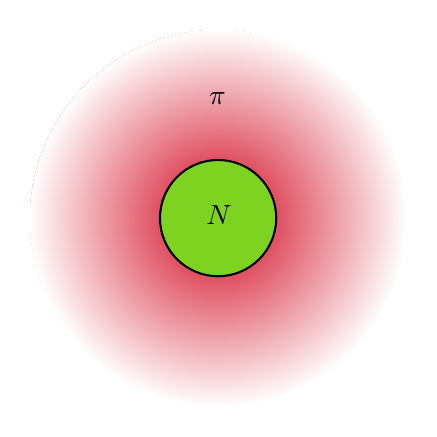
\begin{tikzpicture}[x=0.75pt,y=0.75pt,yscale=-1,xscale=1]
%uncomment if require: \path (0,389); %set diagram left start at 0, and has height of 389

%Flowchart: Connector [id:dp12351893787926194] 
\path  [shading=_3nvmr0jal,_jfsff6evj] (315.75,205) .. controls (315.75,154.6) and (356.6,113.75) .. (407,113.75) .. controls (457.4,113.75) and (498.25,154.6) .. (498.25,205) .. controls (498.25,255.4) and (457.4,296.25) .. (407,296.25) .. controls (356.6,296.25) and (315.75,255.4) .. (315.75,205) -- cycle ; % for fading 
 \draw  [color={rgb, 255:red, 255; green, 255; blue, 255 }  ,draw opacity=1 ][line width=0.75]  (315.75,205) .. controls (315.75,154.6) and (356.6,113.75) .. (407,113.75) .. controls (457.4,113.75) and (498.25,154.6) .. (498.25,205) .. controls (498.25,255.4) and (457.4,296.25) .. (407,296.25) .. controls (356.6,296.25) and (315.75,255.4) .. (315.75,205) -- cycle ; % for border 

%Flowchart: Connector [id:dp2648272257538774] 
\draw  [color={rgb, 255:red, 0; green, 0; blue, 0 }  ,draw opacity=1 ][fill={rgb, 255:red, 126; green, 211; blue, 33 }  ,fill opacity=1 ][line width=0.75]  (379,205) .. controls (379,189.54) and (391.54,177) .. (407,177) .. controls (422.46,177) and (435,189.54) .. (435,205) .. controls (435,220.46) and (422.46,233) .. (407,233) .. controls (391.54,233) and (379,220.46) .. (379,205) -- cycle ;

% Text Node
\draw (399.8,197.6) node [anchor=north west][inner sep=0.75pt]  [color={rgb, 255:red, 0; green, 0; blue, 0 }  ,opacity=1 ]  {$N$};
% Text Node
\draw (401.2,142.8) node [anchor=north west][inner sep=0.75pt]  [color={rgb, 255:red, 0; green, 0; blue, 0 }  ,opacity=1 ]  {$\pi $};


\end{tikzpicture}